\documentclass[a4j,11pt,twoside]{jbook}
\usepackage{ascmac}
\usepackage[dvipdfmx]{graphicx}
\usepackage{matx}
\usepackage{manyfloat}
\begin{document}
%--------------------------------------------
% タイトルページ
\title{倒立振子の安定化制御}
\author{瀧川文哉}
\date{2017年7月}
\maketitle
%--------------------------------------------
% 目次
\pagenumbering{roman}
\tableofcontents
\listoffigures
\listoftables
\cleardoublepage
\pagenumbering{arabic}
%--------------------------------------------
% 本文
\chapter{はじめに}
\section{実験目的}
\section{制御対象と制御目的}
\chapter{モデリング}
\section{数式モデル}
\subsection{状態方程式}
\section{物理パラメータの決定}
\section{パラメータの検証}

\chapter{制御系設計}
\begin{figure}
	\centering
	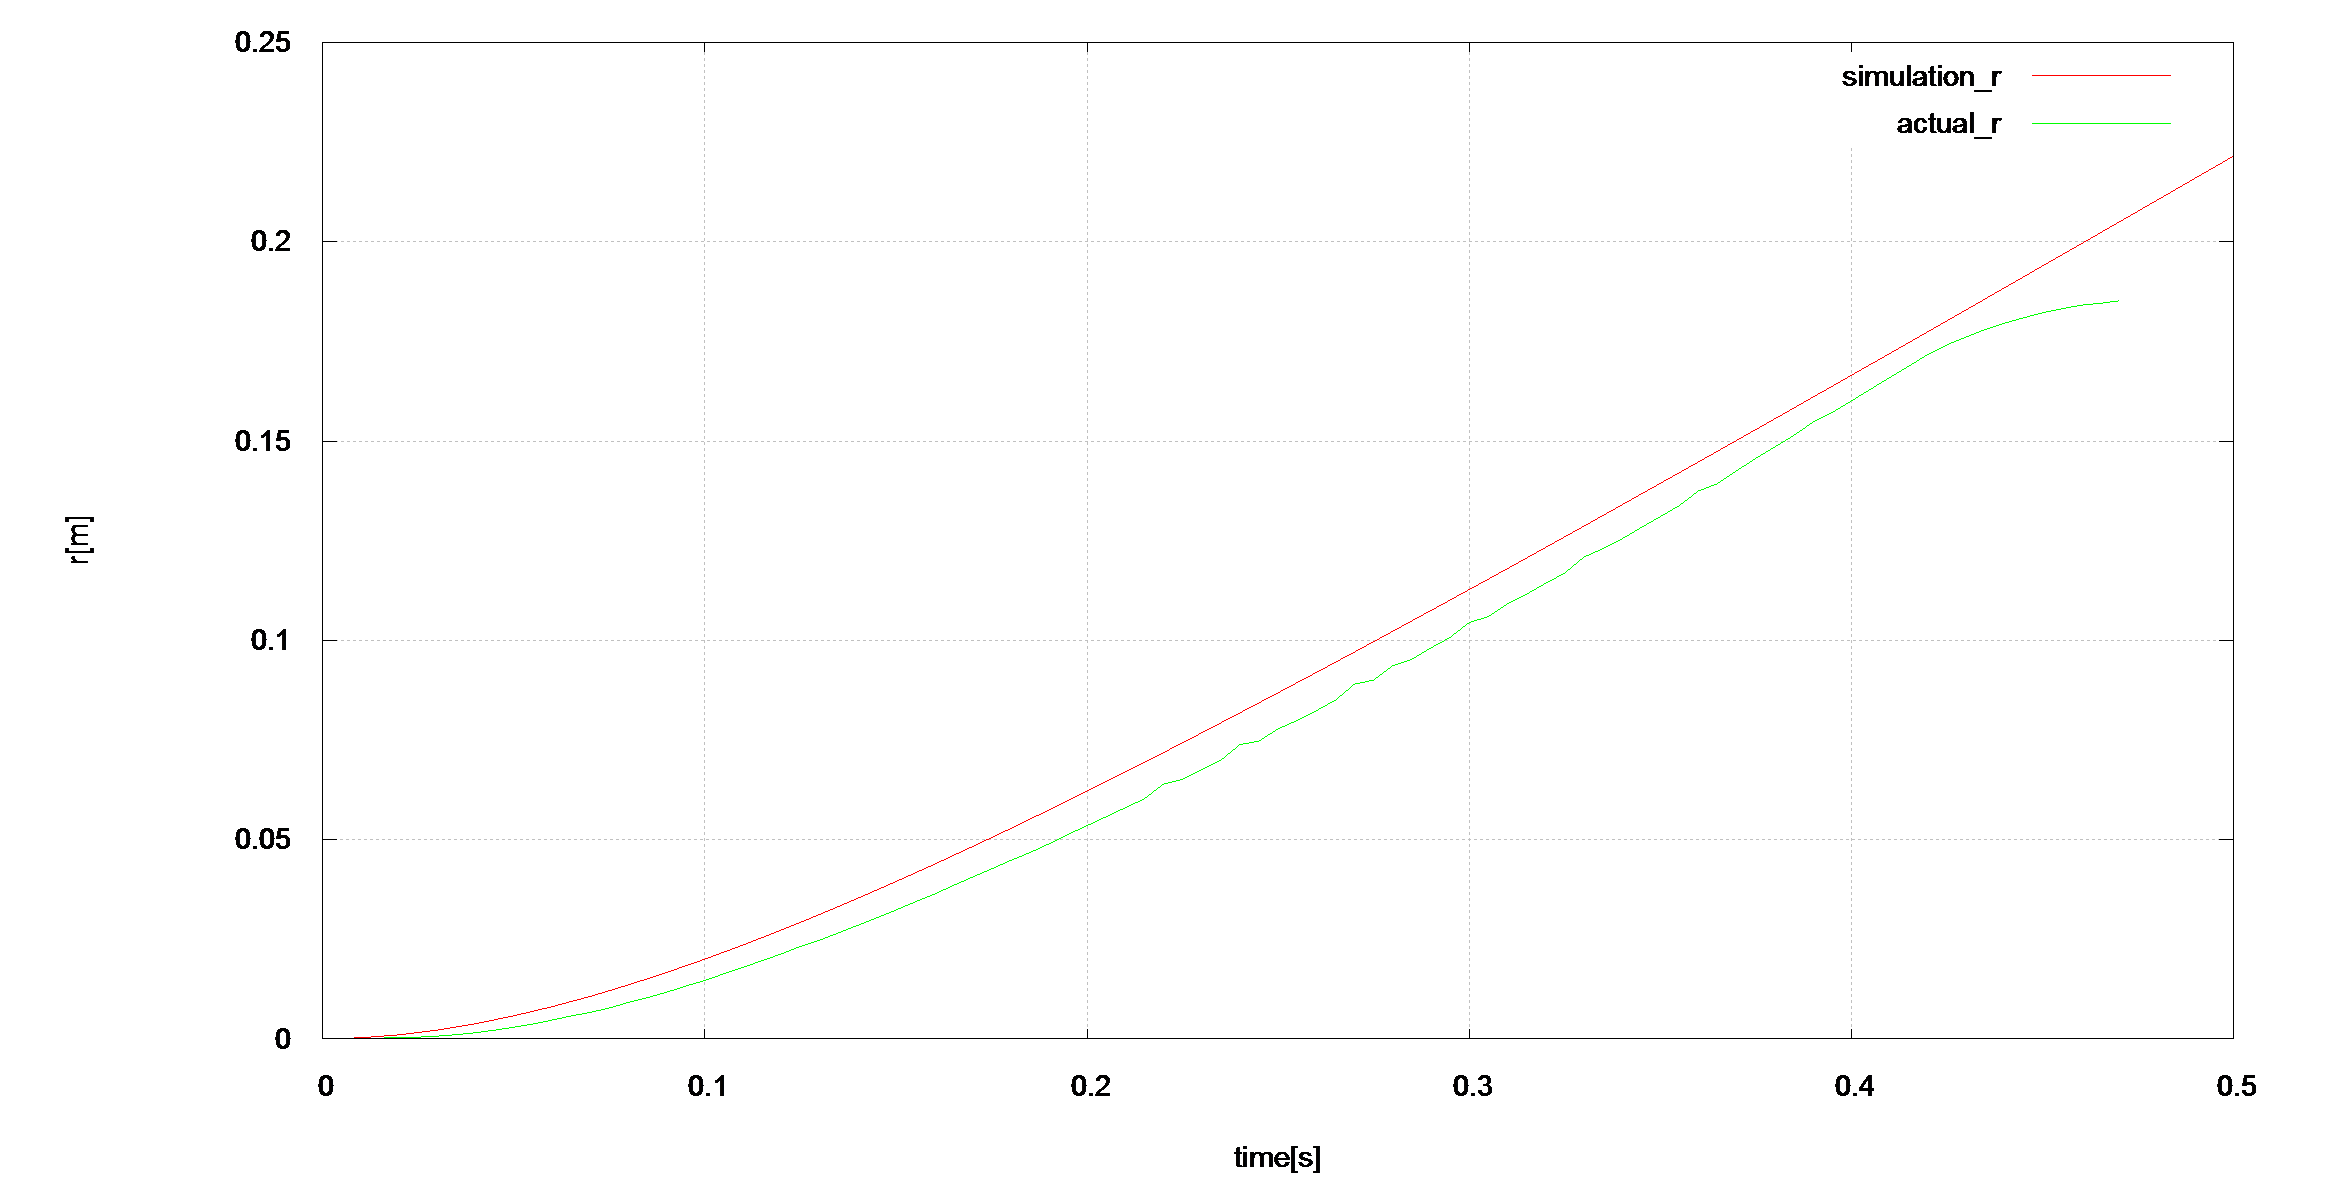
\includegraphics[width=0.7\linewidth]{step11.png}
	\caption{}
	\label{fig:step11}
\end{figure}
\section{特性解析}
\section{制御システムの構成}
\section{$F$の設計}
\section{$\hat{A}$,$\hat{B}$,$\hat{J}$,$\hat{C}$,$\hat{D}$の設計}
\section{離散化}
\section{振り上げ制御}	

\chapter{シミュレーション}
\section{安定化制御}
\section{振り上げ制御}

\chapter{実験}
\section{実験装置}
\section{安定化制御}
\section{振り上げ制御}
\section{考察}

\chapter{おわりに}

\end{document}